\chapter{Background}
\label{chp::background}

This chapter presents an overview of authentication schemes, cryptographic prelims, and identity-based ciphers. Passwords, a human-chosen and memorable secret, forms the foundation of many modern authentication schemes, hence a detail coverage of it here and a dedication of two chapters on why they are guessable (Chapter~\ref{chp4::password-composition}) and how they are guessed (Chapter~\ref{chp5::password-guessing-algorithms}). Identity-based ciphers are used in Chapter~\ref{chp::deeid}; therefore we provide an overview of them here.

\begin{figure}[t]
\noteBox{Protocol}{
A protocol in computing and telecommunications is a set of rules and conventions that govern the exchange of data between devices. It defines the procedures for data transmission, including how data is formatted, transmitted, and received. Protocols ensure that devices can communicate effectively and understand each other, regardless of differences in their underlying hardware or software.
}
\end{figure}

\section{Entity Authentication}
\label{sec::chp2::authentication}

Entity authentication or \textit{identification} is the process of verifying the identity of a user, device, or system before granting access to sensitive information or functionality. It allows the \textit{claimant} to reassure another entity (the \textit{verifier}) of their identity. In related literature~\cite{menezes_handbook_1997}, the terms identification and entity authentication are often used interchangeably. Identification protocols are ubiquitous; we encounter them most commonly when logging into web applications. They are also used when unlocking a car with a wireless key fob or accessing an ATM.

\textbf{Password-based authentication} is the most prevalent form of entity authentication, tracing its history back to the early days of computing. This form of authentication is considered weak due to the vulnerabilities associated with user-chosen passwords. The password itself is a string—often a minimum of six characters—selected and memorised by the user, serving as a shared secret between the user and the system (verifier). The password string is linked to a claim of identity, such as a unique username or email address. We explore password-related topics in depth in Section~\ref{sec::chp2::password}.

\textbf{Personal identification numbers (PINs)} are commonly used on mobile devices or in conjunction with banking cards to prevent unauthorised access to personal devices or other physical possessions. PINs are typically four or six digits long and are most commonly employed as a secondary form of authentication.

Fixed secret schemes, such as passwords and PINs, are susceptible to replay attacks due to eavesdropping. \textbf{One-time passwords (OTPs)} mitigate this risk by ensuring that each password is used only once per login attempt. There are two variants of OTP: (1) Hash-based OTP (HOTP) and (2) Time-based OTP (TOTP). HOTP relies on a counter that increments with each use, whereas TOTP is based on the current time, typically changing every 30 seconds. As a result, TOTP is short-lived and requires only reasonably synchronised clocks, whereas HOTP necessitates synchronisation between both the client and the server. Due to its simplicity and security benefits, TOTP is the more commonly used algorithm.

Protocols that require interaction between entity $A$ (the \textit{claimant}, who is proving their identity) and entity $B$ (the \textit{verifier}) are known as \textbf{challenge-response authentication}. These protocols utilise a time-variant challenge to defend against active attacks; the challenge is provided by entity $B$ (the verifier—a system or device). Kerberos and Needham–Schroeder are examples of symmetric-key, challenge-response-based protocols. We discuss zero-knowledge-based schemes in Section~\ref{sec::chp2::identity-based-ciphers} and utilise them in Chapter~\ref{chp::deeid}.


\section{Attacks on Entity Authentication Protocols}
\label{sec::chp2::attacks-on-auth}

There are various security threats to identification protocols~\cite{menezes_handbook_1997}:  

\begin{itemize}
\item
  \emph{Impersonation}. Pretending to be a different person.
\item
  \emph{Replay attack}. Use of information from a previously used
  protocol process, e.g.~re-use of a poor signature.
\item
  \emph{Interleaving attack}. Multiple concurrent execution of the
  protocol and using selective information for possible attacks.
\item
  \emph{Reflection Attack}. Attack on a challenge-response method to
  essentially tricking the challenger into providing itself with the
  answer.
\item
  \emph{Forced Delay}. Requires intercepting a message and delaying it
  until some later time (thus not a replay attack).
\item
  \emph{Chosen-text Attack}. Strategically choosing challenges in an
  attempt to extract information about the prover's secret information.
\end{itemize}


\section{Multi-Factor Authentication}
\label{chp2::multi-factor-authentication}

\begin{figure}
    \centering
    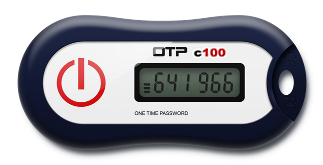
\includegraphics[width=0.33\linewidth]{figs/otp_hardware.jpg}
    \caption{Photograph of a hardware-based OTP device that is capable of generating event-based and time-based one-time passwords. This form is a visual-based hardware OTP as it requires the user to identify the digits and enter them onto another device.}
    \label{fig:otp-hardware}
\end{figure}

Multi-factor authentication (MFA) is a layered approach to security and access control, combining multiple authentication methods to enhance the overall security of a system. Applications typically implement two-factor authentication (2FA), which pairs password-based authentication with an OTP or SMS verification. In practice, OTP methods are commonly implemented through mobile phone applications.

The distinction between what constitutes multi-factor authentication is not always clear-cut. Often, if the \textit{user} is required to interact with multiple systems, it is considered multi-factor authentication. However, when metadata---such as location and IP address---is used, it is less clear whether this qualifies as multi-factor authentication.

Use of multi-factor authentication comes often at a cost to usability. Users are often required to use a secondary device or have access to a mobile phone with LTE access. Use of multi-factor authentication provides additional costs to organisations too--an example of this is when Twitter forced non-paying users to switch from SMS-based 2FA to other forms of 2FA \cite{taylor_twitter_2023}. The reasoning for this was both cost (to Twitter) and the fact that SMS-based 2FA can be vulnerable for most users. The user experience of MFA has hardly changed over the last decade \cite{cristofaro_comparative_2014}, indicating a lack of research or adoption in the research.

The use of multi-factor authentication often comes at the cost of usability. Users are frequently required to utilise a secondary device or have access to a mobile phone with LTE connectivity. Additionally, multi-factor authentication imposes extra costs on organisations---an example of this is when Twitter required non-paying users to switch from SMS-based 2FA to alternative forms of 2FA~\cite{taylor_twitter_2023}. The rationale behind this decision was both the cost to Twitter and the vulnerability of SMS-based 2FA for most users. The user experience of MFA has remained largely unchanged over the past decade~\cite{cristofaro_comparative_2014}, suggesting a lack of research in this area.

SMS-based multi-factor authentication (MFA) involves sending a one-time password (OTP) to the authenticating user via SMS. A mobile phone number is registered to the user's account prior to this authentication stage. However, SMS-based MFA is susceptible to SIM-swapping attacks and SMS interception. Despite these vulnerabilities, SMS-based MFA remains widely adopted due to its convenience and its straightforward usability for users.

One-time passwords (OTPs) are unique authentication secrets generated using a shared secret and are used only once per authentication transaction. Their uniqueness and time-sensitive nature make them resistant to replay attacks. In practice, OTPs are generated through mobile phone applications, dedicated hardware devices, or out-of-band channels.

Hardware tokens are physical devices that generate OTPs. Unlike SMS or app-based OTPs, these tokens operate independently of the user's mobile device or computer—reducing the risk of side-channel attacks. Hardware tokens are also less susceptible to hacking or phishing attacks, as they do not rely on potentially vulnerable network connections. Figure~\ref{fig:otp-hardware} illustrates an example of a hardware-based OTP generator.

\section{FIDO2}
\label{sec::chp2::fido2}

\begin{figure}[t]
    \centering
    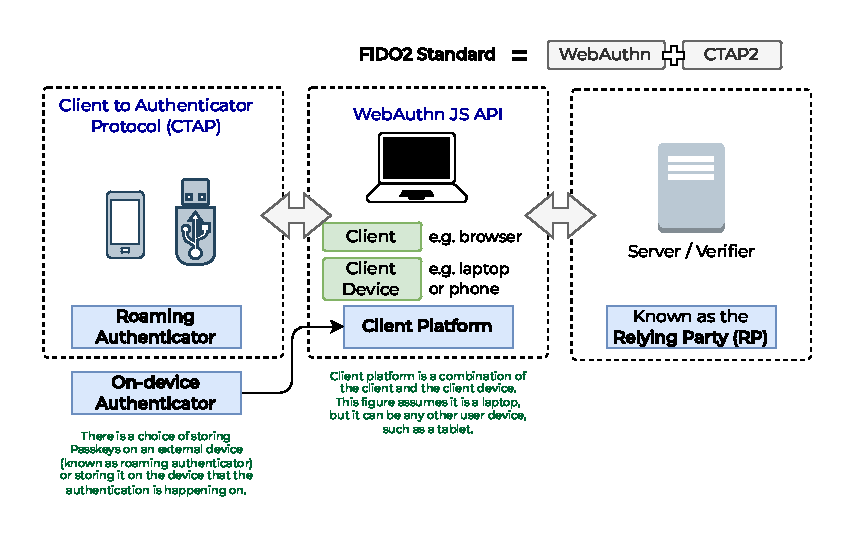
\includegraphics[scale=1.2]{figs/fido2_diagrams.pdf}
    \caption{Diagram showing the core components of the FIDO2 standard. FIDO2's primary intent is to replace password-based authentication with public-key cryptography-based authentication. It consists of the WebAuthn JS API and the protocol to communicate with external devices known as roaming authenticators. \srcOwnFig}
    \label{chp2::fig::fido2-diagram}
\end{figure}

FIDO2 is an authentication standard, which combines the WebAuthn~\cite{noauthor_web_2021} (Web Authentication API) and CTAP2~\cite{noauthor_client_2019} specifications. It represents the primary ongoing effort to replace password-based authentication (i.e., weak authentication) with strong authentication: public-key cryptography-based authentication. It consists of specifications for public-key cryptography-based authentication. Figure~\ref{chp2::fig::fido2-diagram} provides an illustration of the standard's core components.

The credentials in this ecosystem are known as WebAuthn credentials, FIDO credentials, or Passkeys. We will refer to them as Passkeys. Passkeys were introduced by Apple during WWDC 2022~\cite{noauthor_meet_2022} and have attracted considerable attention since then. The advantage of Passkeys for companies like Apple is that they can utilise the biometric features on the device to enhance the authentication experience for the user. However, a drawback is that users are locked into their platforms, as Passkeys are stored on iCloud, or they may lack the knowledge to transfer keys.

The Web Authentication API (WebAuthn)~\cite{noauthor_web_2021} is the specification and JavaScript API developed by W3C and the FIDO Alliance to enable public-key cryptography-based authentication. It is an extension of the Credential Management API. WebAuthn provides the necessary functions to interact with the verifier (server or relying party) and authenticators (which can be on-device or external—roaming authenticators). The Client to Authenticator Protocol (CTAP), currently in version 2 (CTAP2), is the specification that enables authenticators to interact with the WebAuthn API and the client.

FIDO2 is an initiative of the FIDO (Fast IDentity Online) Alliance, an open standard association formed through collaboration among various companies. The association was launched in February 2013 with the aim of creating and promoting a password-less authentication standard within the community. They define their mission as \textit{``authentication standards to help reduce the world's over-reliance on passwords.''} The executive leadership of the alliance includes members from Google, Amazon, Intel, Thales, Apple, Microsoft, and Docomo.

The work of the FIDO Alliance has been hindered by confusion and complexity, leading to a lack of widespread adoption. The maze of specifications, insufficient developer support, and evolving terminologies have made it challenging for developers to implement FIDO2 effectively. The alliance and its output exemplify a design-by-committee approach. Some literature~\cite{farke_you_2020, ghorbani_lyastani_is_2020} has examined the usability of FIDO2 systems in practice, concluding that users often revert to passwords or password managers due to their speed and convenience. Currently, FIDO2 is primarily used for second-factor authentication.

The journey of the FIDO Alliance began with the \texttt{Universal Authentication Framework (UAF)} and \texttt{Universal 2nd Factor (U2F)} standards in 2014. \texttt{Universal 2nd Factor (U2F)} is the standard used to enable two-factor authentication (2FA) through USB HID or NFC. It was succeeded by the Client to Authenticator Protocol 1 (\textbf{\texttt{CTAP1}}) standard, which provides a generalised interaction between the client device and secondary devices.


\section{Secure Hardware}
\label{sec::chp2::secure_hardware}

Isolated hardware with its own operating system can be used to protect user secrets, particularly on mobile phones and wearable devices. These devices store sensitive information such as passwords, financial data, and biometrics, and are ubiquitous; however, they also host numerous untrusted applications that may attempt to access this information. Most importantly, such devices can easily fall into the wrong hands. A response to these threats is dedicated hardware, or a segment of a System-on-Chip (SoC), separated from the rest of the system. This dedicated hardware is referred to as a Trusted Execution Environment (TEE) or a Secure Enclave.

A Trusted Execution Environment (TEE) is a dedicated area of the main processor with its own operating system (for example, on Android, the operating system running on the secure enclave is \fun{Trusty~TEE}~\cite{android_trusty_tee}). The purpose of such architectures is to isolate critical functions and protect cryptographic secrets in isolated contexts (enclaves) from the rest of the system. The remainder of the system is often referred to as the Rich Execution Environment (REE).

Most smartphone manufacturers now build secure enclaves directly into their devices' hardware. Apple design and manufacture their own SoCs and refer to the dedicated secure hardware as the \textit{Secure Enclave}. Other manufacturers, such as Samsung, use ARM-based processors and therefore adopt the \textit{ARM TrustZone} architecture. TEEs in mobile devices store passwords, PINs, biometric data, and other similar secrets. They protect user data by, for example, rate-limiting PIN attempts (with exponential delays) even when a malicious actor has physical access to the device. Biometric data can be stored and processed within the secure enclave; for instance, Touch ID, Face ID, and Optic ID on Apple devices~\cite{apple_biometric_security} are stored and processed exclusively within the secure enclave. On Android, developers can access the TEE via the \fun{Keystore}~API~\cite{android_keystore_api}. Despite the availability of this API, it has been shown~\cite{blessing2025keydroidlargescaleanalysissecure} that most Android applications do not use it for secret storage.

A Hardware Security Module (HSM) is dedicated hardware designed to manage cryptographic secrets. For example, in the cloud, an HSM may be used to avoid loading cryptographic keys into the memory of the main web server. Such isolation prevents leakage and unauthorised access to the keys by other applications.

\section{Topics on Password}
\label{sec::chp2::password}

Passwords are obvious user secrets. Much of this dissertation focuses on human-chosen and memorable secrets, such as \password{il0vesk00l!}, as their weaknesses stem from predictable and frequently used patterns. Password security and authentication constitute a vast field encompassing multiple subfields. Some examples are as follows.


\begin{itemize}
%[itemsep=0pt, parsep=0pt, leftmargin=10pt]
    \item Password usability and user experience
        \begin{itemize}
            \item Password security in enterprise environments
            \item Password creation and memorability
            \item User education and awareness
            \item Password statistics (length, count/freq, structure info)
        \end{itemize}
    \item Password reset and recovery mechanisms
    \item Password modelling and similarity
        \begin{itemize}
            \item Similarity (e.g. distance-like metrics)
        \end{itemize}
    \item Password entropy and complexity analysis 
        \begin{itemize}
            \item Password composition policy (PCP) (or password creation policy)
            \item Password strength meters (PSM)
        \end{itemize}
    \item Password guessing algorithms
    \item Password hashing and encryption techniques
    \item Password-less authentication schemes
    \item Password authentication protocols
    \item Federated identity and single sign-on (SSO)
    \item Biometric and multi-factor authentication
    \item Password-based authentication in specific domains (e.g., web, mobile, IoT)
    \item Password managers and storage
\end{itemize}


\textbf{Statistical and Lexical Password Analysis.} Historical analyses of password characteristics have focused on \textit{length}, \textit{count}, and \textit{character-level structures}~\cite{ma_study_2014, Li_Han_Xu_2014, Das_Bonneau_Caesar_Borisov_Wang_2014, ur_et_al_2015, li_study_2016, pearman_et_al_2017, Pasquini_Cianfriglia_Ateniese_Bernaschi_2021, Cazier_Medlin_2006}. Our research advances this field by examining nuanced aspects of passwords with greater precision. Moreover, the evolution of language models, combined with our successful prototypes, presents a cost-effective approach for labelling additional passwords.

In the analysis of Chinese passwords~\cite{Li_Han_Xu_2014}, the authors conduct a broad examination of password syntax. Our research extends~\cite{Li_Han_Xu_2014} by delving deeper into password structures. For instance, they identified $LLLLLL$ as the predominant structure within the \texttt{Rockyou} dataset, typically representing a word, as demonstrated in our results. Further structural analysis across various password datasets is presented in~\cite{li_study_2016}. Das~\etal~\cite{Das_Bonneau_Caesar_Borisov_Wang_2014} explored password syntax, notably introducing an analysis of word or phrase transformations, which aligns with aspects of our research. However, we disagree with their classification of sequential keys, alternate keys, and sequential alphabets as transformations, instead viewing these as sequences. Riddle~\etal~\cite{Riddle_Miron_Semo_1989} investigate the composition and semantics of passwords, with a particular emphasis on the psychological significance of words.

In ``Investigating the Distribution of Password Choices''~\cite{Malone_Maher_2012}, the analysis of the \hmail dataset concluded that its distribution closely resembles Zipf's law. Our analytical efforts extend this observation by demonstrating that extracted words from unique passwords also follow a similar distribution---more of this is found in Chapter~\ref{chp4::password-composition}.

\textbf{Password Modelling.} Early password modelling techniques, such as the Markov $n$-gram model~\cite{narayanan_fast_2005}, focused on individual characters, positing that \textit{``the distribution of letters in easy-to-remember passwords likely mirrors the letter distribution in the user's native language.''} We validate this in Section~\ref{chp4::password-composition} at the word level. The observation that letter distribution is not uniform holds true for words, exhibiting a power-law distribution akin to Zipf's law. Modelling passwords based on Probabilistic Context-Free Grammars (PCFG)~\cite{weir_password_2009} was the next innovation. Our insights into empirical password structures (\S\ref{sec::chp4::results}) can refine \pcfg modelling. Incorporating $W_n \text{ and } N_n$ as variables for words and names, respectively, enhances the computational viability of modelling more intricate structures. Subsequent advancements have leveraged machine learning techniques in password modelling, including neural networks~\cite{Castro_Lang_Liu_Mata_2017}, GANs~\cite{hitaj_passgan_2019}, RNNs~\cite{Melicher_Ur_Segreti_Komanduri_Bauer_Christin_Cranor_2016}, and Transformers~\cite{Xu_Yu_Zhang_Wang_Zhang_Wu_Han_2023}, among others.

\textbf{Password Composition Policy (PCP).} Despite extensive research into password complexity measures and meters, recommendations for password policies remain scarce. Bonk~\etal~\cite{Bonk_Parish_et_al_2021} provide guidance on constructing passphrases, effectively extending the NCSC's~\cite{ncsc2024} three-word suggestion to longer sequences, such as seven words or more. \zxcvbn employs dictionaries and bespoke rules to gauge password strength on a scale from 0 to 4. However, \zxcvbn has its limitations; for instance, it incorrectly parses the password \password{gomythsun} as \texttt{"go myths un"}, which affects its strength rating. Additionally, it struggles with transformations such as \texttt{"numbr"} from \texttt{"number"}. Wang~\etal~\cite{Wang_Shan_Dong_Shen_Jia_2023} conduct a deeper evaluation of password strength meters. Their endorsement of \zxcvbn and Markov $n$-gram models has informed our research approach.

The deployment of language models, particularly Large Language Models (LLMs), in this domain remains notably scarce. Rando~\etal~\cite{Rando_Perez-Cruz_Hitaj_2023} explored password modelling using the GPT-2 framework. Given the broad embeddings that encompass multiple languages, the semantic breakdown and analysis of passwords represent, in our view, a pioneering application of LLMs.

\section{Computational Hardness Assumptions}

Much of modern security and cryptography is built upon one-way functions—functions that are easy to compute but difficult to invert. The \textit{difficulty} is based on computational and algorithmic efficiency. An algorithm is \textit{efficient} if it runs in polynomial time. More formally, an algorithm is considered efficient if its running time is bounded by a polynomial function of the input size. That is, for an input of size $n$, the running time is $O(n^k)$ for some constant $k$. Cryptographic primitives and protocols are often designed under the assumption that certain computational problems cannot be solved efficiently, i.e., in polynomial time. The hardness of these problems is crucial for maintaining the security of the cryptographic systems based on them. The hypothesis that a problem cannot be solved efficiently is known as the computational hardness assumption.

\textit{Trapdoor one-way function} is a variant of the one-way function that requires a secret key. Using this secret key, one can invert the function; without it, it remains hard to invert.

The existence of one-way functions remains an open conjecture in computer science. However, there are several promising candidates that have withstood attempts at inversion to date. For these functions, no efficient algorithms to compute their inverses have been discovered. Examples of such candidate one-way functions include:

\begin{itemize}
\item \textbf{Integer factorisation problem:} Given a positive integer $n$, find its prime factors. For example, if $n = pq$, where $p$ and $q$ are distinct prime numbers, the factorisation problem is to find $p$ and $q$ given only $n$. Also known as \textit{Factorisation Problem} or simply \textit{Factoring}.

\item \textbf{RSA problem:} The RSA algorithm was the first public key encryption algorithm; though it was also invented by Clifford Cocks at GCHQ in 1973, four years before Rivest, Shamir and Adleman. The RSA problem is finding $m$ given the public key $(n, e)$ and a ciphertext $c \equiv m^e \pmod{n}$. The security of the RSA algorithm is no harder than the integer factorisation problem, so if we can solve the factoring problem, then we can solve the RSA problem. However, there is no proof that solving the RSA problem will help us solve the factoring problem (D. Boneh and R. Venkatesan Breaking RSA may not be equivalent to factoring). Also known as \textit{RSA Assumption} or \textit{RSA Inversion}.

\item \textbf{Quadratic residuosity problem:} Given a composite number $n$ and an integer $a$, determine whether $a$ is a quadratic residue modulo $n$. In other words, find whether there exists an integer $x$ such that $x^2 \equiv a \pmod{n}$.

\item \textbf{Discrete logarithm problem (DLP):} Given a finite cyclic group $G$, a generator $g$ of the group, and an element $h \in G$, find an integer $x$ such that $g^x = h$. The integer $x$ is called the discrete logarithm of $h$ with respect to $g$, denoted as $x = \log_g h$. This problem is considered hard in certain groups, such as the multiplicative group of a finite field or the group of points on an elliptic curve over a finite field.

\item \textbf{Diffie-Hellman problem:} Given a finite cyclic group $G$, a generator $g$ of the group, and elements $g^a$ and $g^b$, where $a$ and $b$ are unknown integers, compute $g^{ab}$. This problem is closely related to the discrete logarithm problem and is used in the Diffie-Hellman key-exchange protocol. The assumption that this problem is hard is known as the Computational Diffie-Hellman (CDH) assumption.
\end{itemize}


Quantum computing does indeed pose a threat to some of the computational hardness assumptions, as quantum computers can solve some problems exponentially faster. Shor's algorithm~\cite{shor_polynomial-time_1997} can solve both the integer factorisation and discrete logarithm problems in polynomial time. This algorithm, for example, threatens RSA- and DLP-based cryptosystems, as it can factor an integer $n$ in $O((\log n)^3)$ time and $O(\log n)$ space.

Post-quantum cryptography deals with finding quantum-resistant problems. For example, \textit{lattice problems} (such as the Shortest Vector Problem) are believed to be quantum resistant. NIST has been actively standardising the process for post-quantum cryptography since 2016. In August 2024, NIST released ML-KEM (CRYSTALS-Kyber) for key establishment. They also released ML-DSA (CRYSTALS-Dilithium) and SLH-DSA (SPHINCS+) for digital signatures. Other national organisations, such as the UK's NCSC, are actively providing guidance to navigate the post-quantum cryptography journey~\cite{ncsc_next_nodate}.

Whilst quantum computers pose a threat to many cryptosystems, it is believed that cryptographic hash functions are quantum resistant. Thus, they do not undermine the security of password-based authentication systems. However, Grover's algorithm~\cite{grover_fast_1996} could aid a malicious user in inverting a function. Grover's algorithm can accelerate unstructured search problems, providing a quadratic speed-up compared to classical algorithms.

\section{Cryptographic Hash Functions}

A hash function is an umbrella term for functions with the following property. A hash function $h$ takes an arbitrary-length input $x$ and outputs $y$, a fixed-length bit string. This is often represented as: $h(x) = y$, where $x$ is the input, message, or preimage, and $y$ is the output, hash value, or hash digest. Table~\ref{tab:hash-functions} shows examples of hash functions and their key properties. In cryptography, we require the hash function to have specific properties for it to be useful. We differentiate it by calling it a cryptographic hash function or a collision-resistant hash function.

Key properties of a cryptographic hash function are as follows.
\begin{itemize}
    \item \textbf{Preimage resistant}: Given a hash value $y$ it should be computationally infeasible to find an input string $x$ such that $y = h(x)$. i.e. it should be computationally infeasible to reverse the hash. Some literature may refer to this property as \textit{one-way property.}
    
    \item \textbf{Second preimage resistant}: Given some input $x_1$ and a hash value $y$, it should be computationally infeasible to find another input $x_2$ that results in the same hash value $y$. Some literature may refer to this property as \textit{weak collision resistant}.
    
    \item \textbf{Collision resistant}: It should be computationally infeasible to find two inputs that result in the same output. Some may refer to this as the \textit{strong collision resistant property}.
\end{itemize}

When designing a hash function, we also require small changes in the input to lead to a large change in the output. This is called the \textit{avalanche effect}.

\begin{table}[t]
    \centering
    \caption{Overview of various hash functions and their key parameters. $n$ is block size in bits and $m$ is output size in bits.}
    \label{tab:hash-functions}
    $$
    \begin{array}{lllllcl}
    \toprule
    \text{Hash function} & n & m & \text{Preimage} & \text{Collision} & \text{Collision Resistant} & \text{Construction} \\
    \midrule
    \text{SHA-1} & 512 & 160 & 2^{160} & 2^{80} & \text{No} & \text{Merkle-Damgård} \\
    \text{SHA-256} & 512 & 256 & 2^{256} & 2^{128} & \text{Yes} & \text{Merkle-Damgård} \\
    \text{SHA-512} & 1024 & 512 & 2^{512} & 2^{256} & \text{Yes} & \text{Merkle-Damgård} \\
    \text{MD5} & 512 & 128 & 2^{128} & 2^{64} & \text{No} & \text{Merkle-Damgård} \\
    \text{RIPEMD-160} & 512 & 160 & 2^{160} & 2^{80} & \text{Yes} & \text{Merkle-Damgård} \\
    \text{Whirlpool} & 512 & 512 & 2^{512} & 2^{256} & \text{Yes} & \text{Miyaguchi-Preneel} \\
    \text{Blake2b} & 1024 & 512 & 2^{512} & 2^{256} & \text{Yes} & \text{HAIFA} \\
    \text{Blake2s} & 512 & 256 & 2^{256} & 2^{128} & \text{Yes} & \text{HAIFA} \\
    \bottomrule
    \end{array}
    $$
\end{table}

Passwords are hashed alongside a unique and random string called a \textit{salt}; this is done per password to prevent \textit{look-up table} or \textit{rainbow-table} attacks. A rainbow table is a precomputed table used for caching the outputs of a cryptographic hash function. A secure method of password storage employs \textit{key derivation functions}. These functions still use one-way functions as primitives but are slower to compute and resistant to rainbow table attacks.

\subsection{Key Derivation Functions}

Key derivation functions (KDFs) are one-way functions that generate cryptographic secret keys from inputs such as passwords. For their use case in password storage and authentication, they offer several advantages over standard cryptographic hash functions. Standard hash functions are designed to be efficient and fast to compute. For password storage, this efficiency makes them insecure, especially as dedicated hardware makes it trivial to compute a large number of hashes per second. This allows an adversary to guess a vast number of passwords. KDFs aim to solve this problem by introducing CPU- and memory-intensive operations, thereby slowing down brute-force and other guessing attacks. Table~\ref{table:password_hash_comparison} shows various KDFs and their key properties.


\begin{definition}[A password-based key derivation function]
    A password-based key derivation function, or PBKDF, is a function H that takes as input a password $w \in \mathcal{P}$, a salt $s \in \mathcal{S}$, and a difficulty $d \in \mathbb{Z}^{>0}$. It outputs a value in ${0,1}^\ell$ for some $\ell$. We require that $H$ is computable by an algorithm that runs in time proportional to $d$. We say that the PBKDF is defined over $(\mathcal{P}, \mathcal{S}, {0,1}^\ell)$.
\end{definition}

\noteBox{NIST's Storage Recommendation}{%
Verifiers SHALL store memorized secrets in a form that is resistant to offline attacks. Memorized secrets SHALL be salted and hashed using a suitable one-way key derivation function. Key derivation functions take a password, a salt, and a cost factor as inputs then generate a password hash. Their purpose is to make each password guessing trial by an attacker who has obtained a password hash file expensive and therefore the cost of a guessing attack high or prohibitive.

Examples of suitable key derivation functions include Password-based Key Derivation Function 2 (PBKDF2) [SP 800-132] and Balloon [BALLOON]. A memory-hard function SHOULD be used because it increases the cost of an attack. The key derivation function SHALL use an approved one-way function such as Keyed Hash Message Authentication Code (HMAC) [FIPS 198-1], any approved hash function in SP 800-107, Secure Hash Algorithm 3 (SHA-3) [FIPS 202], CMAC [SP 800-38B] or Keccak Message Authentication Code (KMAC), Customizable SHAKE (cSHAKE), or ParallelHash [SP 800-185]. The chosen output length of the key derivation function SHOULD be the same as the length of the underlying one-way function output.
}

\begin{table}[t]
\small
\centering
\caption{Overview of various key derivation functions (KDFs) or also some known as Password Hashing Functions.}
\label{table:password_hash_comparison}
\begin{tabular}{crccl}
\toprule
\textbf{Year} & \textbf{Function} & \textbf{Memory-Hard?} & \textbf{Primitive} \\
\midrule
1999 & \texttt{Bcrypt} \cite{provos_future-adaptable_1999} & $\times$ & Blowfish \\
2000 & \texttt{PBKDF2} \cite{kaliski_pkcs_2000} & $\times$ & HMAC \\
2009 & \texttt{Scrypt} \cite{percival_stronger_2009} & $\checkmark$ & Salsa20/8 \\
2013 & \texttt{Catena} \cite{forler_catena_2013} & $\checkmark$ & Blake2b \\
2015 & \texttt{Makwa} \cite{pornin_makwa_2015} & $\times$ & Squaring Modulo \\
2015 & \texttt{yescrypt} \cite{neves_yescrypt_2015} & $\checkmark$ & SHA-256 \\
2015 & \texttt{Argon2} \cite{biryukov_argon2_2016} & $\checkmark$ & Blake2b \\
2015 & \texttt{Lyra2} \cite{andrade_lyra2_2016} & $\checkmark$ & Blake2b \\
2016 & \texttt{Balloon} \cite{boneh_balloon_2016} & $\checkmark$ & Blake2b \\
\bottomrule
\end{tabular}
\end{table}

\textbf{Memory-hard functions} require a large amount of memory to be computed and impose computational penalties if less memory is used. \scrypt\ is one of the first such functions to utilise this approach but suffers from two key vulnerabilities~\cite{forler2014memory}: its password-dependent memory access patterns make it susceptible to cache-timing attacks, and its memory storage approach leaves it vulnerable to garbage-collector attacks, where an adversary can bypass the memory-hardness entirely by recovering stored values after computation. Subsequent key derivation functions, designed with password hashing in mind, aimed to be simpler, resistant to side-channel attacks, and memory-hard. The Password Hashing Competition\footnote{\url{https://www.password-hashing.net/}} was an initiative to accelerate the development of such new functions.

The 2015 Password Hashing Competition gave birth to a host of functions with the following selection criteria\footnote{\url{https://www.password-hashing.net/report-finalists.html}}:
\begin{itemize}
    \item Defense against GPU/FPGA/ASIC attackers
    \item Defense against time-memory tradeoffs
    \item Defense against side-channel leaks
    \item Defense against cryptanalytic attacks
    \item Elegance and simplicity of design
    \item Quality of the documentation
    \item Quality of the reference implementation
    \item General soundness and simplicity of the algorithm
    \item Originality and innovation
\end{itemize}

\argontwo\ was the winner of this competition which provided three variants to mitigate time-memory tradeoff attack: 1) \textit{Argon2d} maximizes resistance to GPU cracking attacks but introduces potential side-channel attacks; 2) \textit{Argon2i} is conversely optimized to resist side-channel attacks; 3) \textit{Argon2id} is a hybrid version of the two prior variants. OWASP \cite{owasp_owasp_2024} recommends using the Argon2id variant with a minimum configuration of 19 MiB of memory, 1 degree of parallelism, and 2 iteration counts. \catena, \lyratwo, \makwa, and \yescrypt\ were the runners up in this competition. \catena\ was developed to address the vulnerabilities of \scrypt by implementing password-independent memory access patterns and providing built-in protection against garbage collection attacks in its double-butterfly graph variant.
% Additionally, \catena\ introduces novel features like client-independent updates and server relief, making it more practical for real-world password hashing applications.

\balloon, developed in 2016, offers several key improvements over existing memory-hard functions like \argontwo. Unlike its predecessors that rely on heuristic security arguments, Balloon provides proven memory-hardness guarantees in the random-oracle model. Its password-independent memory access pattern prevents cache timing side-channel attacks that plague functions like \scrypt, while maintaining competitive performance. The authors demonstrate Balloon's practical advantages by showing an attack against Argon2i that allows computing it with less space than claimed, while Balloon maintains its security properties even under sophisticated analysis.

\noteBox{The OWASP password storage recommendations \cite{owasp_password_2024}}{%
\begin{itemize}
    \item Use Argon2id with a minimum configuration of 19 MiB of memory, an iteration count of 2, and 1 degree of parallelism.
    \item If Argon2id is not available, use scrypt with a minimum CPU/memory cost parameter of ($2^17$), a minimum block size of 8 (1024 bytes), and a parallelization parameter of 1.
    \item For legacy systems using bcrypt, use a work factor of 10 or more and with a password limit of 72 bytes.
    \item If FIPS-140 compliance is required, use PBKDF2 with a work factor of 600,000 or more and set with an internal hash function of HMAC-SHA-256.
    \item Consider using a pepper to provide additional defense in depth (though alone, it provides no additional secure characteristics).
\end{itemize}
}


% \argontwo, the winner of the Password Hashing Competition in 2015, is designed to resist both GPU and ASIC attacks by allowing configuration of memory usage, and CPU processing time. It is defined as follows:
% \[ \texttt{\textbf{Argon2}}\,(\texttt{Password}, \texttt{Salt}, t, m, d, \texttt{len}) \]
% where $t$ is the number of iterations, $m$ is the memory usage in kibibytes, $d$ is the degree of parallelism, and $\text{len}$ is the desired length of the output.
% 





%\subsection{PBKDF2}
%PBKDF2 \cite{kaliski_pkcs_2000} applies a pseudorandom function, such as HMAC-SHA-256, to the input password along with a salt value and repeats the process many times to produce a derived key. The number of iterations, denoted as $c$, is a crucial parameter that enhances the hash's resistance to attacks. The formal definition of PBKDF2 is given by:
%\[ DK = \texttt{PBKDF2}(\texttt{PRF}, \texttt{Password}, \texttt{Salt}, c, \texttt{dkLen}) \]
%where $DK$ is the derived key of length $dkLen$, $PRF$ is the pseudorandom function, and $c$ is the iteration count.


%\subsection{Argon2}
%Argon2 \cite{biryukov_rfc_2021}, the winner of the Password Hashing Competition in 2015, is designed to resist both GPU and ASIC attacks by allowing configuration of memory usage, and CPU processing time. It is defined as follows:
%\[ \texttt{\textbf{Argon2}}\,(\texttt{Password}, \texttt{Salt}, t, m, d, \texttt{len}) \]
%where $t$ is the number of iterations, $m$ is the memory usage in kibibytes, $d$ is the degree of parallelism, and $\text{len}$ is the desired length of the output.
%
%There exist three variants of Argon2:
%\begin{itemize}
%    
%\item \textbf{Argon2d} maximizes resistance to GPU cracking attacks but introduces potential side-channel attacks.
%\item \textbf{Argon2i} is optimized to resist side-channel attacks.
%\item \textbf{Argon2id} is a hybrid version of the two above. It follows the Argon2i approach for the first half pass over memory and the Argon2d approach for subsequent passes. OWASP \cite{owasp_owasp_2024} recommends using this variant with a minimum configuration of 19 MiB of memory, 1 degree of parallelism, and 2 iteration counts.
%\end{itemize}


%If Argon2id is not available, use scrypt with a minimum CPU/memory cost parameter of ($2^17$), a minimum block size of 8 (1024 bytes), and a parallelization parameter of 1.
%For legacy systems using bcrypt, use a work factor of 10 or more and with a password limit of 72 bytes.
%If FIPS-140 compliance is required, use PBKDF2 with a work factor of 600,000 or more and set with an internal hash function of HMAC-SHA-256.
%Consider using a pepper to provide additional defense in depth (though alone, it provides no additional secure characteristics).

%\subsection{Scrypt}
%Scrypt \cite{percival_stronger_nodate} is a password-based key derivation function that is designed to make it costly to perform large-scale custom hardware attacks by requiring large amounts of memory. Its formal definition can be expressed as:
%\[ DK = \text{scrypt}(Password, Salt, N, r, p, dkLen) \]
%where $N$ is the CPU/memory cost factor, $r$ is the block size parameter, $p$ is the parallelization parameter, and $dkLen$ is the length of the derived key.
%
%\subsection{bcrypt}
%bcrypt uses a variant of the Blowfish encryption algorithm and incorporates a salt to protect against rainbow table attacks. It is computationally intensive by design; its key setup phase is slow, which slows down both the attack and normal operations. It can be represented as:
%\[ \text{bcrypt}(Cost, Salt, Input) \]
%where $Cost$ controls the complexity of the underlying algorithm (specifically, the number of hash iterations, represented as $2^\text{Cost}$), $Salt$ is a random value, and $Input$ is the password to be hashed.
%
% \subsection{Preimage Attack}
% A preimage attack, also known as a first preimage attack, is a type of cryptographic attack where an attacker attempts to find a message that produces a given hash value. In other words, given a hash value $h$, the attacker tries to find a message $m$ such that $hash(m) = h$. This attack is considered successful if the attacker can find any message that produces the given hash value.
% Preimage attacks are computationally difficult for secure hash functions, as they are designed to be one-way functions. The complexity of a preimage attack is typically $2^n$, where $n$ is the bit length of the hash digest. For example, finding a preimage for a 256-bit hash digest would require $2^{256}$ hash computations on average, which is considered infeasible with current computing power.
% 
% \subsection{Birthday Attack}
% A birthday attack, also known as a collision attack, is a type of cryptographic attack that exploits the birthday paradox to find collisions in hash functions. The birthday paradox states that in a group of 23 people, there is a 50\% probability that two people share the same birthday. Similarly, in a birthday attack, the attacker tries to find two different messages that produce the same hash digest.
% 
% The complexity of a birthday attack is lower than that of a pre-image attack. The number of hash computations required for a successful birthday attack is approximately $\sqrt{2^n}$, where $n$ is the bit length of the hash digest. For example, finding a collision for a 256-bit hash digest would require approximately $2^{128}$ hash computations, which is significantly less than the $2^{256}$ computations required for a pre-image attack.
%To mitigate the risk of birthday attacks, hash functions used for cryptographic purposes, such as digital signatures and password storage, should have a sufficiently large output size. Increasing the hash digest length reduces the probability of collisions and makes birthday attacks more computationally intensive.




\section{Identity-based Cryptosystems}
\label{sec::chp2::identity-based-ciphers}

\begin{table}[]
    \small
    \centering
    \caption{Table of Identity-based cryptosystems.}
    \label{tab:my_label}
\begin{tabular}{cccc}
\toprule
\textbf{Year} & \textbf{Protocol} & & \textbf{Type} \\
\midrule
1984 & Shamir & \cite{shamir_identity-based_1984} & Signature \\
1986 & Fiat--Shamir & \cite{fiat_how_1986} & Identification \\
1988 & Feige--Fiat--Shamir & \cite{feige_zero-knowledge_1988} & Identification \\
1988 & GQ & \cite{guillou_practical_1988} & Identification \\
1988 & Beth & \cite{beth_efficient_1988} & Identification \\
1990 & Schnorr & \cite{schnorr_efficient_1990} & Identification \\
1991 & Ong--Schnorr & \cite{ong_fast_1991} & Signature \\
1991 & Girault & \cite{girault_identity-based_1991} & Identification \\
1993 & Okamoto & \cite{okamoto_provably_1993} & Identification \\
2002 & Choon--Cheon & \cite{choon_identity-based_2002} & Signature \\
2004 & Ateniese--Medeiros & \cite{ateniese_identity-based_2004} & Hash \\
2005 & Kurosawa--Heng & \cite{kurosawa_identity-based_2005} & Identification \\
2009 & Chin--Heng--Goi & \cite{chin_hierarchical_2009} & Identification \\
2011 & Tan--Heng--Phan--Goi & \cite{tan_variant_2011} & Identification \\
2020 & Chia--Chin & \cite{chia_identity_2020} & Identification \\
\bottomrule
\end{tabular} 
\end{table}

Identity-based cryptosystems or protocols are a type of public-key cryptography where a user's public key is derived directly from some unique identifier of the user, such as their email address, domain name, or phone number. They are \textit{challenge-response} identification protocols and are considered to be strong authentication. Challenge-response identification involves a prover (or claimant) $A$ authenticating to a verifier (or challenger) $B$. 

% The drawbacks of using a public-key-based ciphers or digital signatures are its practicality, certification and trusted party requirements. Such drawbacks are mitigated in identity-based identification protocols. It essentially allows one to use one's identity (e.g.~name, date of birth, place of birth etc.) as a public-key. In such a system everyone would have access to some function \(f\). This function would allow one to compute the public-key from some string which is unique to the individual.

The protocols to be discussed in this section are zero-knowledge protocols. A protocol (or proof system) has the \textit{zero-knowledge property} if it is an \textit{interactive proof system} where the verifier learns nothing beyond the validity of the assertion being proved. These \textit{interactive proof systems} have the following general structure:

\begin{enumerate}
    \item $A \rightarrow B:$ witness
    \item $A \leftarrow B:$ challenge
    \item $A \rightarrow B:$ response
\end{enumerate}

Adi Shamir first introduced an identity-based signature scheme in his seminal 1984 paper, ``Identity-based cryptosystems and signature schemes'' \cite{shamir_identity-based_1984}. This approach remains grounded in public-key cryptosystems but incorporates a distinctive modification. Instead of generating and publishing a traditional public key, users can utilise a set of unique personal identifiers (e.g., name, date of birth, place of birth) as a substitute for the public key. 

Shamir only provides a signature implementation scheme for his identity-based system idea. Shamir returns to this idea in subsequent papers in the years following 1984. In 1986, Fiat and Shamir present the first concrete solution~\cite{fiat_how_1986}. They note that \emph{``The new identification scheme is a combination of zero-knowledge interactive proofs~\cite{goldwasser_knowledge_1985} and identity-based schemes~\cite{shamir_identity-based_1984}.''} In this paper~\cite{fiat_how_1986}, they provide both the signature and proof-of-identity scheme that Shamir proposed in his 1984 paper~\cite{shamir_identity-based_1984}. Moreover, Shamir, along with Feige and Fiat, produces a further study on \emph{``Zero-Knowledge Proofs of Identity''}~\cite{feige_zero-knowledge_1988}. This paper discusses and differentiates between zero-knowledge \emph{``proofs of membership''} and \emph{``proofs of knowledge.''}

\subsection{Feige--Fiat--Shamir Identification Protocol}

This is the protocol as described in \textit{``Zero Knowledge Proofs of identity''} \cite{feige_zero-knowledge_1988}. We have made some adjustments to the notation to keep it consistent throughout this dissertation. Its security depends on the intractability of computing the square roots mod n.

Assuming the interaction is occurring between two entities, the \textit{prover $A$} and the \textit{verifier $B$}.

\textbf{$A$'s key generation protocol is as follows:}

\begin{enumerate}
    \item Choose $k$ random numbers $S_1,...,S_k$ in $\mathbb{Z}_n$
    \item Choose each $v_j$ (randomly and independently) as $\pm1 \cdot (S_j^2)^{-1} \mod{n}$
    \item Publish $v_1,...,v_k$ and keep $S_1,...,S_k$ secret
\end{enumerate}

\textbf{The generation and verification process (i.e. interactions) takes place as follows through a four-step process:}
Repeat \(t\) times:

Repeat steps 3 to 6 for \(i = 1, \ldots, t\):

\begin{enumerate}
    \setcounter{enumi}{2}
    \item $A$ picks a random \(r_i \in [0, n)\) and sends \(x_i = r_i^2 \pmod{n}\) to $B$.
    \item $B$ sends a random binary vector \((e_{i1}, \ldots, e_{ik})\) to $A$.
    \item $A$ sends to $B$:
    \[
    y_i = r_i \prod_{e_{ij}=1} s_j \pmod{n}.
    \]
    \item B checks that
    \[
    x_i \equiv y_i^2 \prod_{e_{ij}=1} v_j \pmod{n}.
    \]
\end{enumerate}


In their final remarks~\cite{feige_zero-knowledge_1988}, Feige, Fiat, and Shamir note: \emph{``An interesting modification can eliminate the public key directory and lead to a key-less identification scheme.''} We use the identity string to public-key transformation provided in~\cite{feige_zero-knowledge_1988} to create public keys in the system.

There are other protocols similar to the Fiat--Shamir protocol, such as the Guillou--Quisquater (GQ) identification scheme~\cite{guillou_practical_1988}, which differs by reducing the number of messages exchanged and the memory requirements for user secrets. The Schnorr identification protocol~\cite{schnorr_efficient_1990} relies on the intractability of the discrete logarithm problem, unlike the Fiat--Shamir and GQ protocols.
%\section{Web Security Attacks}
\label{sec::chp2::security-attacks}

%TODO: OSI layer attacks
%\begin{table}[h!]
\footnotesize
\centering
\begin{tabular}{|c|l|}
\hline
\textbf{OSI Layer} & \textbf{Attack Types} \\
\hline
\multirow{5}{*}{Physical (Layer 1)} & Wiretapping \\
 & Eavesdropping \\
 & Cable cutting \\
 & Electromagnetic interference (EMI) \\
 & Power fluctuations \\
\hline
\multirow{5}{*}{Data Link (Layer 2)} & MAC spoofing \\
 & ARP spoofing \\
 & VLAN hopping \\
 & STP (Spanning Tree Protocol) attacks \\
 & CDP (Cisco Discovery Protocol) attacks \\
\hline
\multirow{7}{*}{Network (Layer 3)} & IP spoofing \\
 & ICMP flooding \\
 & Smurf attack \\
 & Ping of Death \\
 & Teardrop attack \\
 & IP fragmentation attacks \\
 & Routing attacks (e.g., BGP hijacking) \\
\hline
\multirow{5}{*}{Transport (Layer 4)} & SYN flooding \\
 & TCP session hijacking \\
 & UDP flooding \\
 & Port scanning \\
 & Firewalk attack \\
\hline
\multirow{4}{*}{Session (Layer 5)} & Session hijacking \\
 & Session fixation \\
 & NetBIOS attacks \\
 & RPC (Remote Procedure Call) attacks \\
\hline
\multirow{3}{*}{Presentation (Layer 6)} & ASN.1 (Abstract Syntax Notation One) attacks \\
 & Data encoding attacks \\
 & Format string attacks \\
\hline
\multirow{12}{*}{Application (Layer 7)} & Cross-site scripting (XSS) \\
 & SQL injection \\
 & Remote code execution \\
 & Buffer overflow \\
 & Denial of Service (DoS) \\
 & Man-in-the-Middle (MitM) attacks \\
 & Phishing attacks \\
 & Malware (viruses, worms, Trojans) \\
 & Brute-force attacks \\
 & Directory traversal attacks \\
 & Injection flaws \\
 & Insecure direct object references \\
 & Broken authentication and session management \\
\hline
\end{tabular}
\caption{Different types of attacks against each of the OSI layers}
\label{tab:osi-layer-attacks}
\end{table}

This section provides an overview of malicious techniques used for unauthorised exploitation of web applications (not exclusively) and exfiltration of user secrets. We will refer to some of these attacks through the thesis. The main purpose is for this section to act as a reference and guide. This is a comprehensive version of the OWASP's list of attacks. https://owasp.org/www-community/attacks/

Seldom is a single threat vector used exclusively in the real world. Often, multiples areas of weaknesses are exploited to complete a mission. Therefore, having a broad perspective of these attacks and their relationships with each other is essential.


\subsection{Client Side Attacks}
\label{chp2::client-side-attacks}

\textbf{\textsc{Credential Stuffing Attack.}} Attackers use Credential Stuffing Attack (CSA) to gain unauthorised account and system access. They do this by using compromised login information from previous data breaches. CSA owes its success to the inherent weaknesses in the Password. Such weaknesses include: re-using passwords across different systems and using weak passwords.

The increasing number of data breaches has made this form of attack viable. The heap of data that is often dumped on the internet increases the feasibility of CSA. This accelerating threat has led to the likes of SEC issuing warnings to the industry \cite{noauthor_secgov_2020}.

CSA is one of the many consequences of dumped private data. Others include identity fraud and attempted blackmailing by emailing the victims of the data breaches \cite{noauthor_scam_2020}.

\textbf{\textsc{Man-in-the-Browser.}} MitB is usually a Trojan that infects a system and its applications (typically a browser). Once it infects a browser or an operating-system (OS) it can read network traffic, inject code into web pages, change HTTP headers, and generally manipulate the web page for the benefit of the attacker \cite{noauthor_man---browser_2020}. MitB Trojans are also referred to as \emph{Financial Trojans} because (typically) their aim is commit fraud and steal money from their victims. Such malicious actions are done by form grabbing banking details, personal details and changing transaction details (if the user is using online banking to transfer money).

One of the oldest and most famous MitB Trojan is ZeuS \cite{noauthor_zeus_2010}, also known as Zbot. First discovered in 2006, it has caused vast amount of financial damages. Its creator reportedly retired in 2010 and released \cite{noauthor_zeus_2011} its source code to ZeuS' competitor, SpyEye \cite{noauthor_trojan.spyeye_nodate}.

Despite improvements in browser and OS security, criminals are finding
creative ways in penetrating user systems in order to commit malicious
activities.

Mobile phones are not safe either. A variant of ZeuS known as Zitmo \cite{etaher_zeus_2015} or The-Zeus-in-the-Mobile targets mobile phone
devices.

Form grabbing is a type of MitB that has one focus: to skim and steal
contents of forms that the user is filling out. Form grabbers are often
malicious JavaScript code running on compromised websites.

MitB malware is prevalent in the financial sector and payment gateway
systems. Using this method, the attackers maximise their financial gain.
A notable example of MitB---in the form of form grabbing--- is the
British Airways' incident: the attackers were able to manipulate a
third-party JavaScript running on British Airways' payment page. This
manipulation allowed them to scrape payment data as they were entered on
the site by British Airways' customers \cite{klijnsma_british_2018}.

\textbf{\textsc{Password Spraying Attack.}}

%   \begin{figure}[H]
%           \centering
%           \textbf{Authentication with explicit link to deeID}
%           \begin{sequencediagram}
%               \centering
%               \newinst[1]{A}{User}
%               \newinst[1]{B}{Client}
%               \newinst[1]{C}{Server}
%               \newinst[1]{D}{Attacker}
%               \mess{D}{Infect JS Skimmer}{C}
%               \mess{B}{GET /payment}{C}
%               \mess{C}{Respond /payment}{B}
%               \mess{A}{Type payment data $= d$}{B}
%               \mess{A}{Press Submit}{B}
%               \mess{B}{POST /m, body $= d$}{D}
%               \mess{B}{POST /payment, body $= d$}{C}
%           \end{sequencediagram}
%           \label{seq:basicmitb}
%           \caption{Sequence of a basic MitB Skimmer.}
%       \end{figure}

\begin{enumerate}
\def\labelenumi{\arabic{enumi}.}
\item
  \textbf{Clickjacking or UI Redress Attack}: This is a deceptive technique where a
  malicious website or attacker tricks a user into clicking on something
  different from what they perceive. It is typically done by overlaying
  transparent elements on a legitimate webpage, making users perform
  unintended actions without their knowledge.
\item
  \textbf{Cross Frame Scripting (XFS)}:  This is an attack that combines malicious JavaScript with an iframe that loads a legitimate page in an effort to steal data from an unsuspecting user. This attack is usually only successful when combined with social engineering. An example would consist of an attacker convincing the user to navigate to a web page the attacker controls. The attacker’s page then loads malicious JavaScript and an HTML iframe pointing to a legitimate site. Once the user enters credentials into the legitimate site within the iframe, the malicious JavaScript steals the keystrokes.
\item
  \textbf{Cross Site History Manipulation (XSHM)}: XSHM is an attack
  that manipulates the browser's history to change the URLs visited by a
  user. This can lead to confusing and potentially harmful navigation,
  exploiting the same-origin policy of web browsers.
\item
  \textbf{Cross Site Tracing}: Cross Site Tracing is an attack that
  takes advantage of HTTP TRACE requests to steal sensitive information,
  often through cross-site scripting or other vulnerabilities. It can
  expose cookies or credentials to attackers.
\item
  \textbf{Mobile code invoking untrusted mobile code}: This refers to
  situations where mobile code (code executed on a mobile device, like a
  smartphone) invokes other untrusted code, which could potentially lead
  to security risks. It's a concern in the context of mobile app
  development.
\item
  \textbf{Mobile code non-final public field}: This relates to the
  exposure of non-final public fields in mobile code, which can be
  manipulated or tampered with by external parties, potentially leading
  to security vulnerabilities.
\item
  \textbf{Mobile code object hijack}: In this attack, malicious mobile
  code can hijack or take control of objects or resources in a mobile
  environment, potentially leading to unauthorized access or
  manipulation.
\item
  \textbf{Qrljacking}: Qrljacking is a type of attack where an attacker
  tricks users into scanning a QR code that leads to a malicious website
  or action, rather than the intended destination.
\item
  \textbf{Reflected DOM Injection}: Reflected DOM Injection is a type of
  cross-site scripting (XSS) attack where the injected script
  manipulates the Document Object Model (DOM) of a web page. This can
  lead to various security issues and data theft.
\item
  \textbf{Reverse Tabnabbing}: Reverse Tabnabbing is a variant of
  phishing that occurs when a malicious website changes the content of a
  previously opened tab or window, making it appear legitimate while
  tricking the user into revealing sensitive information.
\item
  \textbf{Cross-Site Scripting (XSS)}: XSS is a widespread attack where
  an attacker injects malicious scripts into web content that is then
  executed by unsuspecting users. It can result in data theft, session
  hijacking, or defacement of websites. It can occur in various
  contexts, including in subtitles, if not properly sanitized.
\item
  \textbf{Cross Site Request Forgery (CSRF)}: CSRF is an attack where an
  attacker tricks a user into unknowingly making an unwanted request to
  a different website on which the user is authenticated, potentially
  causing unauthorized actions.
\item
  \textbf{Drive-By Downloads}: Drive-By Downloads are attacks that
  automatically download and install malicious software onto a user's
  device when they visit a compromised or malicious website, often
  without their consent.
\item
  \textbf{Browser Fingerprinting}: Browser fingerprinting is a technique
  used to collect unique information about a user's web browser and
  device. This information can be used to track users without their
  knowledge, compromising privacy.
\item
  \textbf{Content Spoofing - Form Spoofing}: Content spoofing,
  particularly form spoofing, involves manipulating the content of web
  forms to deceive users into providing sensitive information to a
  malicious website or attacker.
\item
  \textbf{Malvertising}: Malvertising involves delivering malicious
  software or content through online advertisements. Users may
  unknowingly encounter malware by clicking on these ads.
\item
  \textbf{Session Fixation}: Session fixation is an attack where an
  attacker sets or fixes a user's session identifier, potentially
  allowing them to impersonate the victim after login.
\item
  \textbf{Malicious Browser Extensions}: Malicious browser extensions
  are browser add-ons or plugins that appear harmless but can steal
  data, inject ads, or compromise user privacy.
\end{enumerate}

%TODO: Server side attacks
%\subsection{Server-Side Attacks}

\begin{itemize}
\item \textbf{Binary Planting:} Uploading and executing unauthorized binary files on the server, usually a specific location. Binary planting can be used to escalate privileges. An example of this is the Stuxnet virus using the  Microsoft Windows Print Spooler Service Remote Code Execution Vulnerability (CVE-2010-2729 / BID 43073). Also known as \textbf{DLL Planting} or \textbf{DLL Hijacking}.
\item \textbf{SQL Injection}
\begin{itemize}
    \item Blind SQL Injection: Extracting data from a database by sending queries and observing the server's response time or behavior.
\end{itemize}
\item Blind XPath Injection: Extracting data from an XML document by sending queries and observing the server's response time or behavior.
\item Buffer Overflow via Environment Variables: Manipulating environment variables to cause a buffer overflow and execute arbitrary code.
\item Buffer Overflow Attack: Overwriting memory beyond the bounds of a buffer to corrupt data or execute arbitrary code.
\item \textbf{CORS}
\begin{itemize}
    \item CORS Origin Header Scrutiny: Exploiting misconfigured Cross-Origin Resource Sharing (CORS) headers to access restricted resources.
    \item CORS Request Preflight Scrutiny: Exploiting misconfigured CORS preflight requests to bypass security checks.
\end{itemize}
\item \textbf{File Injection:}
\begin{itemize}
    \item CSS 
    \item CSV Injection: Injecting malicious payloads into CSV files to execute arbitrary code or perform unauthorized actions.
\end{itemize}

\item Cache Poisoning: Manipulating cached data to serve malicious content to users.
\item Cash Overflow: Manipulating financial calculations to cause integer overflows and perform unauthorized transactions.
\item Code Injection: Injecting malicious code into a vulnerable application to execute arbitrary commands or manipulate data.
\item Command Injection: Executing arbitrary commands on the server by injecting them into vulnerable input fields.
\item Comment Injection Attack: Injecting malicious comments or code into an application's data store or output.
\item Content Spoofing: Tricking users into believing that malicious content is legitimate by mimicking the appearance of a trusted website.
\item Custom Special Character Injection: Injecting special characters into input fields to bypass validation or cause unintended behavior.
\item Denial of Service (DoS): Overwhelming a server with requests to exhaust its resources and make it unavailable to users.
\item Direct Dynamic Code Evaluation - Eval Injection: Injecting malicious code into an application's eval() function to execute arbitrary commands.
\item Embedding Null Code: Injecting null bytes into input fields to bypass validation or manipulate file paths.
\item Execution After Redirect (EAR): Executing malicious code after a redirect to bypass security checks.
\item Forced Browsing: Accessing restricted pages or resources by guessing or manipulating URLs.
\item Form Action Hijacking: Modifying the action attribute of HTML forms to submit data to an attacker-controlled server.
\item Format String Attack: Exploiting format string vulnerabilities to read or write arbitrary memory locations.
\item Full Path Disclosure: Revealing the full path of files or directories on the server.
\item Function Injection: Injecting malicious code into a vulnerable function to execute arbitrary commands or manipulate data.
\item HTTP Response Splitting: Injecting newline characters into HTTP headers to split the response and insert malicious content.
\item LDAP Injection: Injecting malicious LDAP queries to extract sensitive information or manipulate directory services.
\item Log Injection: Injecting malicious payloads into application logs to execute arbitrary code or manipulate log data.
\item Server-Side Includes (SSI) Injection: Injecting SSI directives to execute arbitrary commands or include malicious files.
\item Server-Side Request Forgery (SSRF): Tricking a server into making unauthorized requests to internal or external resources.
\item Session Prediction: Guessing or predicting valid session identifiers to hijack user sessions.
\item Session Fixation: Forcing a user to use a predefined session identifier to hijack their session.
\item Session Hijacking Attack: Stealing or predicting session identifiers to take over user sessions.
\item Setting Manipulation: Modifying application settings or configuration files to alter its behavior or gain unauthorized access.
\item Special Element Injection: Injecting special elements or tags into input fields to bypass validation or manipulate the application's behavior.
\item Unicode Encoding: Exploiting Unicode encoding vulnerabilities to bypass input validation or inject malicious payloads.
\item Web Parameter Tampering: Manipulating URL parameters or form data to perform unauthorized actions or bypass security checks.
\item Windows ::DATA Alternate Data Stream: Hiding malicious files or data in alternate data streams on Windows systems.
\item XML External Entity (XXE) Injection: Exploiting XML parsers to access unauthorized files or network resources.
\item XPath Injection: Injecting malicious XPath queries to extract sensitive information from XML documents.
\item Cross-Site Request Forgery (CSRF): Tricking users into performing unintended actions on a web application in which they are authenticated.
\item Web Service Amplification Attack: Exploiting web services to amplify denial of service attacks by sending large amounts of data.
\end{itemize}


\hypertarget{other-attacks}{%
\subsubsection{Other Attacks:}\label{other-attacks}}

\begin{itemize}
\item
  Brute Force Attack
\item
  Cross-User Defacement
\item
  Forced browsing
\item
  Form action hijacking by Robert Gilbert (amroot)
\item
  Man-in-the-browser attack
\item
  Manipulator-in-the-middle attack
\item
  Parameter Delimiter
\item
  Path Traversal
\item
  Regular expression Denial of Service - ReDoS by Adar Weidman
\item
  Repudiation Attack
\item
  Resource Injection
\item
\begin{verbatim}
* **Inband**. The same channel is used to inject SQL code and extract sensitive data.
\end{verbatim}
\item
\begin{verbatim}
* **Out-of-band.**  Data is retrieved using a different channel.
\end{verbatim}
\item
\begin{verbatim}
* **Inferential.**  Gaining information from behaviour server based on sent requests.
\end{verbatim}
\item
\begin{verbatim}
* Tools:
\end{verbatim}
\item
\begin{verbatim}
    * mieliekoek.pl
\end{verbatim}
\item
\begin{verbatim}
    * wpoison
\end{verbatim}
\item
\begin{verbatim}
    * sqlmap
\end{verbatim}
\item
\begin{verbatim}
    * wapiti
\end{verbatim}
\item
\begin{verbatim}
    * w3af
\end{verbatim}
\item
\begin{verbatim}
    * paros
\end{verbatim}
\item
\begin{verbatim}
    * sqid
\end{verbatim}
\item
\begin{verbatim}
* User input
\end{verbatim}
\item
\begin{verbatim}
* Cookies
\end{verbatim}
\item
\begin{verbatim}
* HTTP Headers
\end{verbatim}
\item
\begin{verbatim}
* Second-order SQL Injections
\end{verbatim}
\item
  Traffic flood
\item
  Trojan Horse
\item
  Unicode Encoding
\item
  Windows ::DATA Alternate Data Stream
\end{itemize}